\chapter{多目标、对抗与双层优化}
\label{chap:multiobjective-minimax-bilevel}

前面固定了比较候选的标量目标，只改变求解方法。本章处理三种“最优答案”的含义本身发生变化的任务：多个指标互相竞争时需要规定如何取舍（多目标），两方选择方向相反时需要规定响应次序（极小极大），评价依赖另一个优化问题的解时需要规定内层怎样选解（双层）。三者不共用同一种最优性标准、收敛率或计算成本。

\section{多目标优化}

若同时关心预测精度与计算时间，一个数无法同时概括两项指标。给非空可行集$C$与全部要最小化的向量目标$\bm f=(f_1,\ldots,f_m):C\to\mathbb R^m$，先定义比较关系。

\begin{definition}[支配与Pareto最优]
\label{def:opt-pareto-optimality}
若$\bm u,\bm v\in C$满足所有$i$都有$f_i(\bm u)\leq f_i(\bm v)$且至少一项严格小，称$\bm u$\term{支配}（dominate）$\bm v$。不被任何可行点支配的点称为\term{Pareto最优}（Pareto optimal）；只要求不存在所有分量都严格更小的点，则称弱Pareto最优。
\end{definition}

目标像$\bm f(C)$中不被支配的部分称Pareto前沿；参数空间的Pareto集合与目标像中的前沿是不同对象。

\subsection{加权和法}

权重把偏好落实成一个标量：
\[
 \min_{\bm w\in C}\sum_i\alpha_i f_i(\bm w),\qquad
 \alpha_i\geq0,\quad\sum_i\alpha_i=1.
\]
权重确定后即可调用前文章节匹配的标量方法，并报告全部原指标。所有权重严格为正时，标量问题的全局最小点必为Pareto最优：支配它的候选会使加权和严格更小；允许零权时一般只保弱Pareto。加权和只选择被权重方向支撑的前沿点。三个可行损失向量$(0,1),(1,0),(0.6,0.6)$互不支配，第三点是Pareto最优，但任意权重下前两点至少一个值不超过$0.5<0.6$，所以加权和永远不选它——非凸（或非下凸包）前沿上存在未支撑Pareto点。

图~\ref{fig:opt-pareto-weighted-sum}标出三点与一条支撑等值线。
\begin{figure}[htbp]
  \centering
  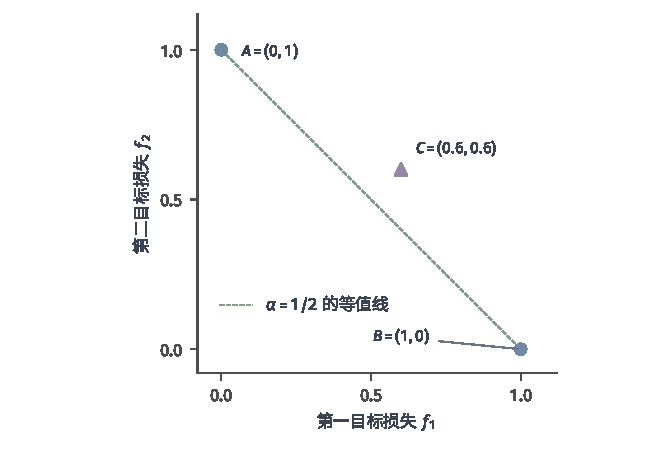
\includegraphics[width=112.0mm]{figures/00-shared/mathematical-preliminaries-upper/04-optimization/matplotlib/opt-pareto-weighted-sum/figure.pdf}
  \caption{三个精确可行损失向量。$A,B,C$互不支配，但对任意$\alpha\in[0,1]$，$C$的加权损失$0.6$都严格大于$\min\{\alpha,1-\alpha\}$；绿虚线为$\alpha=1/2$时通过$A,B$的等值线。Pareto最优不保证能由加权和选到。}
 \label{fig:opt-pareto-weighted-sum}
\end{figure}

\subsection{最小范数梯度组合法}

若当前希望同时改善所有指标，方向$\bm d$满足
\[
 \langle\nabla f_i(\bm w),\bm d\rangle<0\quad(\forall i)
\]
时称为\term{共同下降方向}的严格版本。把原点投影到梯度凸包上：
\[
 \bm\alpha^\star\in\arg\min_{\bm\alpha\in\bm\Delta_m}
 \frac12\left\|\sum_i\alpha_i\nabla f_i(\bm w)\right\|_2^2,
 \qquad
 \bar{\bm g}=\sum_i\alpha_i^\star\nabla f_i(\bm w).
\]
权重子问题是单纯形约束凸二次问题，凸包紧故投影向量$\bar{\bm g}$唯一（权重未必唯一）。

\begin{theorem}[无共同下降方向的一阶判定]
\label{thm:opt-common-descent}
对可微的$m$个目标，无约束点$\bm w$处不存在共同严格下降方向，当且仅当存在$\alpha_i\geq0$、$\sum_i\alpha_i=1$使$\sum_i\alpha_i\nabla f_i(\bm w)=\bm0$。
\end{theorem}

\begin{proof}
若零凸组合存在而$\bm d$使每个内积为负，加权内积也为负，矛盾。反之，若原点不在梯度凸包内，凸集外点分离给出与每个梯度内积同号的方向，必要时取反即为共同严格下降方向。
\end{proof}

若$\bar{\bm g}\neq\bm0$，投影最优性给$\langle\bar{\bm g},\nabla f_i-\bar{\bm g}\rangle\geq0$，取$\bm d=-\bar{\bm g}$则每个方向导数至多$-\|\bar{\bm g}\|^2$；各目标$L_i$光滑时$0<\eta<2/\max_iL_i$使这一步共同下降，未知常数时要求每个目标都通过回溯。例$f_1=((x-1)^2+y^2)/2$、$f_2=((x+1)^2+y^2)/2$在$(0,1)$的梯度为$(-1,1),(1,1)$，最小范数平均$(0,1)$、步长$1$到$(0,0)$，两项各降$1/2$；在$(0,0)$零已在两梯度之间，不能再共同下降。该判据只排除一阶共同改善（两目标均为$-x^2$在$0$处即为反例），有约束时还要限制方向可行。

\subsection{阈值约束法与有限候选实现}

若某些指标有硬上限，保留一个指标作目标、其余写成约束：
\[
 \min\{f_j(\bm w):\bm w\in C,\ f_i(\bm w)\leq B_i\ (i\neq j)\}.
\]
其全局最小点至少弱Pareto最优（全部指标严格更小的候选会连$f_j$一起改善），但未必Pareto，需要时在最优候选中再排除支配点。

\paragraph{有限候选的码率—失真选择。}
给有限方案的码率$R_k$、失真$D_k$（均越小越好），预算题枚举$\min\{D_k:R_k\leq B\}$，价格题枚举$\min_k(D_k+\lambda R_k)$。把三点$(R,D)=(0,1),(1,0),(0.6,0.6)$用于$B=0.6$：第三点以$D=0.6$入选，而任何$\lambda$都不选它——预算题与价格题覆盖不同答案。点间线段只有在混合实际允许（编码块或时间可拼接）并计入拼接成本时才有可行含义；若总代价可加且各块独立，固定$\lambda$时$\min\sum_i(D_i+\lambda R_i)=\sum_i\min(D_i+\lambda R_i)$，但总预算约束仍耦合各块。只有在另外建立了可由支撑线达到的光滑下降曲线$D(R)$后，内部最优才满足$D'(R)+\lambda=0$；不对有限点的角点直接求导。概率率失真函数还需信息论前提。

\subsection{原多目标问题的最优性与解集}

定理~\ref{thm:opt-common-descent}是算法无关的一阶证书；它不保证全局Pareto最优。若每个目标凸，零梯度凸组合使相应加权和全局最小，给弱Pareto结论；严格正权重再加强为Pareto。$f_1(x)=0,f_2(x)=x^2$在$x=1$满足一阶判据却被$x=0$支配，说明零权的边界。非空紧可行集与连续指标下，严格正权标量目标的全局最小点存在且Pareto最优，保证至少有一个Pareto点；紧性负责达到，正权负责排除支配。

\subsection{进展、敏感性与预算}

加权和沿指定偏好求解、不保证每项逐轮下降；最小范数法在合格条件下保证当前共同下降，零向量只给一阶证书；有限枚举在给定候选与预算内返回最小失真。改变权重时标量解可连续移动，改变预算时答案可在$R_k$跨过阈值处离散切换。枚举、标量求解与梯度子问题各有成本，回溯还要对每个指标重复评价。

\section{极小极大优化}

在鲁棒训练的一个样本$(\bm x,y)$上，固定参数$\bm w$后考虑允许集合$\Delta$中的特征扰动$\bm\delta$；标签$y$不变。若$\Delta$非空紧、损失关于$\bm\delta$连续，内层最大值达到，外层再降低这种最坏损失。一般形式为
\begin{equation}
 \min_{\bm w\in W}\max_{\bm z\in Z}\phi(\bm w,\bm z).
 \label{eq:opt-minimax}
\end{equation}
外层先选$\bm w$，内层看到它后选使损失最大的$\bm z$；外层最小化的是最坏响应值，交换次序一般改变值。

\subsection{鞍点、间隙与最值交换}

\begin{definition}[极小极大鞍点]
\label{def:opt-minimax-saddle}
点$(\bm w^\star,\bm z^\star)$若对所有$\bm w\in W,\bm z\in Z$满足
\[
 \phi(\bm w^\star,\bm z)\leq\phi(\bm w^\star,\bm z^\star)
 \leq\phi(\bm w,\bm z^\star),
\]
称为\term{极小极大鞍点}（minimax saddle point）。
\end{definition}

这是两组变量承担相反优化方向时的全局最优响应关系，不是多元微积分中由Hessian正负曲率定义的微分鞍点。定义
\[
 P(\bm w)=\sup_{\bm z\in Z}\phi(\bm w,\bm z),\qquad
 D(\bm z)=\inf_{\bm w\in W}\phi(\bm w,\bm z),
\]
总有$D(\bm z)\leq P(\bm w)$，非负的\term{原始--对偶间隙}$P(\bm w)-D(\bm z)$为零时该候选对满足鞍点不等式。

\begin{theorem}[紧凸凹条件下的最值交换]
若$W,Z$非空、紧且凸，$\phi$连续，对固定$\bm z$关于$\bm w$凸、对固定$\bm w$关于$\bm z$凹，则
\[
 \min_{\bm w\in W}\max_{\bm z\in Z}\phi
 =\max_{\bm z\in Z}\min_{\bm w\in W}\phi,
\]
且两侧最值均达到。
\end{theorem}

证明思路（完整分离论证较长）：任取$c$小于左侧值，紧性给出有限个$\bm z_1,\ldots,\bm z_k$使每个$\bm w$至少在一项超过$c$；考虑由这些值定义的向上封闭凸集，严格分离给出非负归一权重，再用关于$\bm z$的凹性把加权响应合成为$Z$中一个$\bar{\bm z}$，推出右侧值大于$c$；令$c$趋于左侧值并结合弱对偶即得等号，连续性保证两侧达到。紧性、连续性与凸凹性各司其职，一般非凸对抗训练不能直接套用。

\subsection{同时梯度下降—上升法}

在可微延拓下，两方在同一旧点各取一次偏梯度：
\[
 \bm w^+=\Pi_W(\bm w-\eta\nabla_{\bm w}\phi(\bm w,\bm z)),\qquad
 \bm z^+=\Pi_Z(\bm z+\eta\nabla_{\bm z}\phi(\bm w,\bm z)).
\]
两方向都从同一旧点计算。取$W=Z=[-1,1]$、$\phi(x,z)=xz$：$P(x)=|x|$、$D(z)=-|z|$，唯一鞍点$(0,0)$，候选间隙为$|x|+|z|$。不投影时
\[
 (x^+)^2+(z^+)^2=(1+\eta^2)(x^2+z^2),
\]
每个非零初值向外旋转（离开盒后已不是可行候选）。加盒投影也不收敛：$\eta=1$从$(1,0)$出发沿八个角点和边中点周期循环，间隙始终不小于$1$。值的存在定理不替代具体算法的收敛定理。

\subsection{外梯度法}

外梯度先试探、再用试探点方向从旧点校正：
\[
 \bar{\bm u}=\Pi_K(\bm u-\eta\bm F(\bm u)),\qquad
 \bm u^+=\Pi_K(\bm u-\eta\bm F(\bar{\bm u})),
\]
其中$\bm u=(\bm w,\bm z)$、$\bm F(\bm u)=(\nabla_{\bm w}\phi,-\nabla_{\bm z}\phi)$、$K=W\times Z$，每轮两次方向求值与两次投影。在双线性例中投影未激活时更新矩阵为$\begin{smallmatrix}1-\eta^2&-\eta\\ \eta&1-\eta^2\end{smallmatrix}$，距离平方每步乘
\[
 1-\eta^2+\eta^4<1\qquad(0<\eta<1).
\]
取$\eta=1/2$、$\|\bm u^{(0)}\|_2\leq1/2$：试探点范数至多$\sqrt5/4<1$、校正点范数递减，归纳得两次投影都不激活且距离几何收缩，故趋于鞍点、间隙趋零。这是该例的可核验改善；一般问题还需梯度映射的单调性、Lipschitz等条件，多算一次方向本身不是普遍收敛定理。

图~\ref{fig:vol1-add-minimax-rotation}比较两种更新的轨迹与距离。
\begin{figure}[!htb]
  \centering
  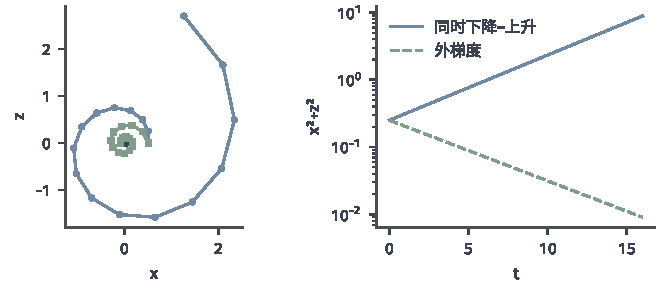
\includegraphics[width=112mm]{figures/00-shared/mathematical-preliminaries-upper/00-shared/matplotlib/mathematical-language-combinatorics-analysis-optimization-comprehension-additions/minimax-rotation.pdf}
  \caption{对$\phi(x,z)=xz$取$\eta=1/2$、初值$(1/2,0)$。蓝线为无投影同时下降--上升，距离平方每步乘$1+\eta^2$；绿线为外梯度，每步乘$1-\eta^2+\eta^4<1$。蓝线离盒后不是可行候选，绿线试探与校正始终在盒内。}
  \label{fig:vol1-add-minimax-rotation}
\end{figure}

\subsection{结果、过程与预算}

紧凸凹条件保证值交换与鞍点达到，却不指定轨迹；同一双线性盒任务上同时法循环、外梯度在特定初值与步长内收缩，故存在性与算法收敛分别报告。比较预算时同时法每轮两组偏梯度，外梯度每轮两次求值加两次投影；若全局间隙还需内层最优响应，其求解成本也要计入。

\section{双层优化}
\label{sec:opt-bilevel}

\term{双层优化}中，有些决策必须先经过一次学习才能评价：外层变量$\bm\theta\in\Theta\subseteq\mathbb R^p$（如正则强度）先改变内层训练问题，训练后参数再给外层损失。令内层变量$\bm w\in\mathbb R^d$。若内层有多个最小点，只写$\bm w^\star(\bm\theta)\in\arg\min_{\bm w}L_{\rm in}$没有定义单值映射，可规定乐观（取外层值下确界）或悲观（上确界）选解，或给定由初始化与算法决定的选择规则$S$。下文假设内层最小解唯一或已给定单值选择：
\[
 \bm w^\star(\bm\theta)=S(\bm\theta)\in\arg\min_{\bm w}L_{\rm in}(\bm w,\bm\theta),
\]
外层实际比较的是内层选解经过评价后的复合目标
\begin{equation}
 J(\bm\theta)=L_{\rm out}(\bm w^\star(\bm\theta),\bm\theta).
 \label{eq:opt-bilevel-objective}
\end{equation}
例$L_{\rm in}(w,\theta)=(w^2-1)^2$的内层最小点恒为$\{-1,1\}$，外层$(w-\theta)^2/2$在$\theta=1$时乐观值$0$、悲观值$2$：内层最优值相同不消除外层歧义。内层最大化可改写为最小化负目标；鲁棒训练的内外层角色（内层选扰动、外层调参数）与超参调优不同，不能套用同一说明。

\subsection{迭代展开法}

\subsubsection{梯度下降的展开与外层方向}

对内层更新$\bm w^{(t+1)}=\bm w^{(t)}-\eta\nabla_{\bm w}L_{\rm in}(\bm w^{(t)},\bm\theta)$（二阶连续可微、固定步长），定义
\[
 \bm A^{(t)}=\bm I-\eta\nabla_{\bm w,\bm w}^2L_{\rm in},\qquad
 \bm B^{(t)}=\nabla_{\bm w,\bm\theta}^2L_{\rm in},
 \qquad
 \bm D_t=\frac{\mathrm d\bm w^{(t)}}{\mathrm d\bm\theta},
\]
则$\bm D_{t+1}=\bm A^{(t)}\bm D_t-\eta\bm B^{(t)}$。有限步目标$J_T(\bm\theta)=L_{\rm out}(\bm w^{(T)}(\bm\theta),\bm\theta)$的外层梯度为
\[
 \nabla_{\bm\theta}J_T
 =\bm D_T^\top\nabla_{\bm w}L_{\rm out}
 +\nabla_{\bm\theta}L_{\rm out}.
\]
存储大时等价地反向累计：保存$\bm q_T=\nabla_{\bm w}L_{\rm out}$，逆向做$\bm h\leftarrow\bm h-\eta(\bm B^{(t)})^\top\bm q_{t+1}$、$\bm q_t=(\bm A^{(t)})^\top\bm q_{t+1}$，再加初值依赖项。

\subsubsection{带历史状态、截断与数值核验}

带动量等优化器时展开对象须是完整状态$\bm z^{(t)}=(\bm w^{(t)},\bm s^{(t)})$：$\bm D_z^{t+1}=(\partial_{\bm z}\mathcal U_t)\bm D_z^t+\partial_\theta\mathcal U_t$；符号、裁剪分支与平方根切换处要检查复合映射的可微范围。前向仍跑$T$步、只截断反向$\ell$步，舍去的是Jacobian乘积，方向误差不超过$\|\nabla_{\bm w}L_{\rm out}\|\,\|\bm A^{T-1}\cdots\bm A^{T-\ell}\|\,\|\bm D_{T-\ell}\|$；而减少前向步数改变的是$J_T$本身。用$L_{\rm in}=(w-\theta)^2/2$、$w^{(0)}=0$、$\eta=1/2$：两步得$w^{(2)}=3\theta/4$，外层$(w-1)^2/2$在$\theta=2$的梯度为$3/8$；理想内层解$w^\star=\theta$对应梯度为$1$。两者都正确，差别在求导对象——点收敛不自动推出导数收敛。

图~\ref{fig:opt-bilevel-target-chains}把这两个目标的计算链放在同一画面中。有限步链把两次实际更新纳入复合函数，理想链则直接使用精确内层解；二者即使共享内层损失与外层评价，导数也对应不同的目标。

\begin{figure*}[htbp]
 \centering
 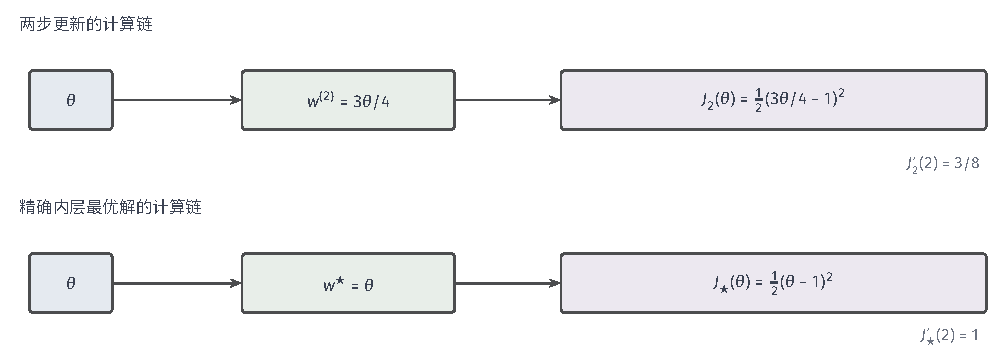
\includegraphics[width=168.998mm]{figures/00-shared/mathematical-preliminaries-upper/04-optimization/tikz/opt-bilevel-target-chains/figure.pdf}
 \caption{同一二次内层目标的两条计算链。固定$w^{(0)}=0$、步长$1/2$，两次更新产生$w^{(2)}=3\theta/4$；精确最优解则为$w^\star=\theta$。外层都读取$(w-1)^2/2$，但两个复合目标不同，故在$\theta=2$处分别得到导数$3/8$与$1$。有限步算法的求导与精确解分支的求导各自对应自己的目标。}
 \label{fig:opt-bilevel-target-chains}
\end{figure*}

\subsection{隐式微分法}

\subsubsection{选定分支的可微性与目标归属}

固定局部最小点$\widehat{\bm w}_0$（无约束内点），其满足$\nabla_{\bm w}L_{\rm in}=\bm0$。若$\bm H_{ww}=\nabla_{\bm w,\bm w}^2L_{\rm in}$可逆，隐函数定理给出局部可微驻点分支；非退化局部最小点处$\bm H_{ww}\succ\bm0$，分支保持严格局部最小。但隐函数定理不承担全局归属：只有该分支始终是规定的全局选解，才有$\widehat J=J$；Hessian奇异是局部导数问题，分支非凸不全局最优是目标归属问题，提高求解精度都不能修复。

\subsubsection{隐式导数、伴随计算与两类残差}

对驻点方程关于$\bm\theta$求导：
\[
 \bm H_{ww}\widehat{\bm D}+\bm H_{w\theta}=\bm0
 \quad\Longrightarrow\quad
 \widehat{\bm D}=-\bm H_{ww}^{-1}\bm H_{w\theta},
\]
代入外层链式法则得\term{隐式超梯度}
\begin{equation}
 \nabla_{\bm\theta}\widehat J
 =\nabla_{\bm\theta}L_{\rm out}
 -\bm H_{w\theta}^\top\bm H_{ww}^{-\top}\nabla_{\bm w}L_{\rm out},
 \label{eq:opt-implicit-hypergradient}
\end{equation}
实践中解伴随方程$\bm H_{ww}^\top\bm v=\nabla_{\bm w}L_{\rm out}$而不显式求逆。

近似内层点的残差$\bm r_{\rm in}=\nabla_{\bm w}L_{\rm in}(\widetilde{\bm w},\bm\theta)$在邻域$\bm H_{ww}\succeq\mu\bm I$下给点误差$\|\widetilde{\bm w}-\widehat{\bm w}\|\leq\|\bm r_{\rm in}\|/\mu$；同点线性系统残差$\bm r_{\rm lin}=\widetilde{\bm H}^\top\widetilde{\bm v}-\widetilde{\bm g}$给伴随误差。设超梯度作为$\bm w$的函数在该邻域Lipschitz常数为$C$，总误差满足
\begin{equation}
 \|\widetilde{\nabla_{\bm\theta}\widehat J}
 -\nabla_{\bm\theta}\widehat J\|_2
 \leq\frac{C}{\mu}\|\bm r_{\rm in}\|_2
 +\frac{\|\widetilde{\bm B}\|_2}{\mu}\|\bm r_{\rm lin}\|_2.
 \label{eq:opt-hypergradient-two-residuals}
\end{equation}
两项分别来自内层点不准与同点伴随未解准；小$\mu$同时放大二者。取得外层方向后仍要按$\widehat J$的光滑性和可行集执行自己的步长与停止。

\subsection{原双层问题的选解、结果与预算}

原双层问题的外层最小点存在要逐参数核验：内层适当下半连续且有紧下水平集时内层解达到，适当闭强凸给内层唯一，但这些不自动给外层最小点，还需选解规则连续、外层损失连续与参数域紧等条件。结果评价先固定针对$J_T$、$\widehat J$还是$J$：展开法给有限步目标的导数，隐式法给合格分支的导数，$3/8$与$1$不是数值误差而是不同目标的正确导数。总预算比较须合计前向内层迭代、存储或重算、反向传播、伴随求解与外层迭代；压低一种残差未必控制完整超梯度误差。

\section{本章小结}

多目标先用支配排除共同劣势，再用权重、共同方向或阈值规定取舍；梯度凸包含零只是一阶证书，未支撑Pareto点与有限工作点不能被加权和自动覆盖。极小极大先规定响应次序，用全局鞍点不等式与候选间隙检验输出；紧凸凹使最值可交换，但同时下降--上升仍可能旋转，外梯度的收缩依赖额外条件。双层先规定内层选解，再区分有限步目标$J_T$、局部分支$\widehat J$与理想全局选解$J$；展开梯度与隐式超梯度各自忠实于其目标，内层驻点残差与伴随残差要同时控制。最优化部分至此覆盖了问题定义、存在与最优性、光滑与非光滑求解、约束证书、预算近似与决策结构；后续函数空间章将把有限维参数推广到函数，随机逼近与策略评价则会复用本章的对偶与鞍点语言。
